\documentclass[border=5pt]{standalone}
\usepackage{tikz}
\usepackage{tcolorbox}
\usepackage{varwidth}
\usepackage{amssymb}
\usetikzlibrary{positioning, fit, backgrounds, shapes.geometric}

\definecolor{promptbg}{RGB}{240,248,255}
\definecolor{rulebg}{RGB}{255,250,205}
\definecolor{taskbg}{RGB}{255,240,245}
\definecolor{outputbg}{RGB}{245,255,245}
\definecolor{bordercol}{RGB}{70,130,180}

\begin{document}

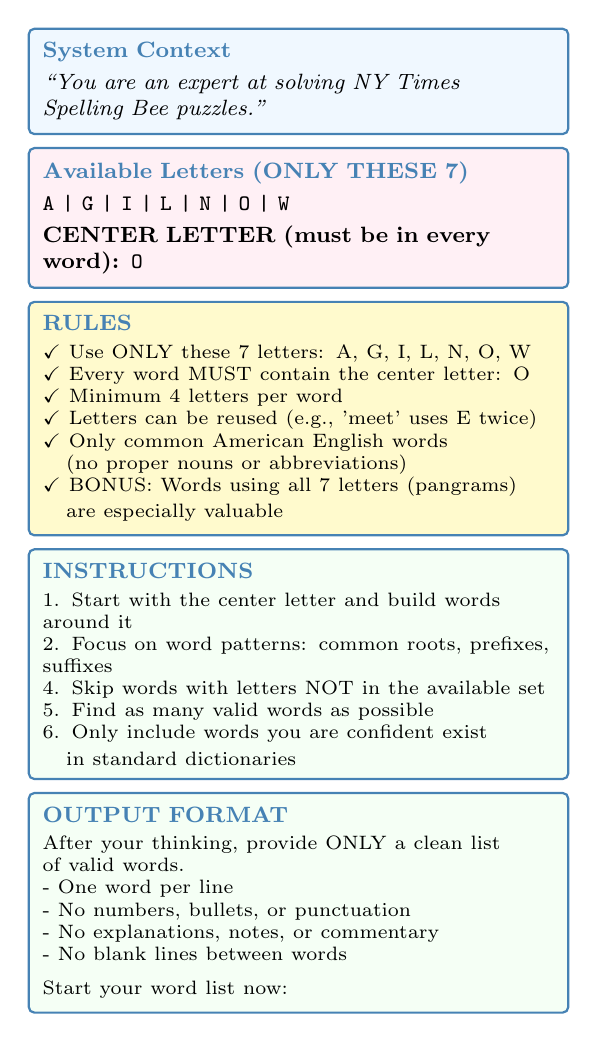
\begin{tikzpicture}[
    box/.style={
        rectangle,
        rounded corners=2pt,
        draw=bordercol,
        line width=0.8pt,
        text width=6.5cm,
        align=left,
        inner sep=5pt,
        font=\footnotesize
    }
]

% System Context
\node[box, fill=promptbg] (system) at (3.25, 0) {
    \textcolor{bordercol}{\textbf{System Context}}\\[2pt]
    \textit{``You are an expert at solving NY Times}\\
    \textit{Spelling Bee puzzles.''}
};

% Current Puzzle
\node[box, fill=taskbg, below=0.15cm of system] (task) {
    \textcolor{bordercol}{\textbf{Available Letters (ONLY THESE 7)}}\\[2pt]
    \texttt{A | G | I | L | N | O | W}\\[2pt]
    \textbf{CENTER LETTER (must be in every word):} \texttt{O}
};

% Rules Section
\node[box, fill=rulebg, below=0.15cm of task] (rules) {
    \textcolor{bordercol}{\textbf{RULES}}\\[2pt]
    {\scriptsize
    $\checkmark$ Use ONLY these 7 letters: A, G, I, L, N, O, W\\
    $\checkmark$ Every word MUST contain the center letter: O\\
    $\checkmark$ Minimum 4 letters per word\\
    $\checkmark$ Letters can be reused (e.g., 'meet' uses E twice)\\
    $\checkmark$ Only common American English words\\
    \hspace{0.3cm}(no proper nouns or abbreviations)\\
    $\checkmark$ BONUS: Words using all 7 letters (pangrams)\\
    \hspace{0.3cm}are especially valuable
    }
};

% Instructions Section
\node[box, fill=outputbg, below=0.15cm of rules] (instructions) {
    \textcolor{bordercol}{\textbf{INSTRUCTIONS}}\\[2pt]
    {\scriptsize
    1. Start with the center letter and build words around it\\
    2. Focus on word patterns: common roots, prefixes, suffixes\\
    4. Skip words with letters NOT in the available set\\
    5. Find as many valid words as possible\\
    6. Only include words you are confident exist\\
    \hspace{0.3cm}in standard dictionaries
    }
};

% Output Format Section
\node[box, fill=outputbg, below=0.15cm of instructions] (output) {
    \textcolor{bordercol}{\textbf{OUTPUT FORMAT}}\\[2pt]
    {\scriptsize
    After your thinking, provide ONLY a clean list\\
    of valid words.\\
    - One word per line\\
    - No numbers, bullets, or punctuation\\
    - No explanations, notes, or commentary\\
    - No blank lines between words\\[3pt]
    Start your word list now:
    }
};

\end{tikzpicture}

\end{document}

